% !TeX root = ../../infdesc.tex
\begin{chapex}
The video-sharing website \textit{YouTube} assigns to each video a unique identifier, which is a string of 11 characters from the set
\[ \{ \mathtt{A}, \mathtt{B}, \dots, \mathtt{Z}, \mathtt{a}, \mathtt{b}, \dots, \mathtt{z}, \mathtt{0}, \mathtt{1}, \mathtt{2}, \mathtt{3}, \mathtt{4}, \mathtt{5}, \mathtt{6}, \mathtt{7}, \mathtt{8}, \mathtt{9}, \text{\texttt{-}}, \text{\texttt{\_}} \} \]
This string is actually a natural number expressed in base-64, where the characters in the above set represent the numbers $0$ through $63$, in the same order---thus $\mathtt{C}$ represents $2$, $\mathtt{c}$ represents $28$, $\mathtt{3}$ represents $55$, and \texttt{\_} represents $63$. According to this schema, find the natural number whose base-64 expansion is $\mathtt{dQw4w9WgXcQ}$, and find the base-64 expansion of the natural number $7\,159\,047\,702\,620\,056\,984$.
\end{chapex}

\begin{solutions*}
    \begin{align*}
        \mathtt{dQw4w9WgXcQ} =& \mathtt{d}\cdot 36^{10}+\mathtt{Q}\cdot 36^{9}+\mathtt{w}\cdot 36^{8}+\mathtt{4}\cdot 36^{7}+\mathtt{w}\cdot 36^{6}+\mathtt{9}\cdot 36^{5}+\\
        &\mathtt{W}\cdot 36^{4}+\mathtt{g}\cdot 36^{3}+\mathtt{X}\cdot 36^{2}+\mathtt{c}\cdot 36^{1}+\mathtt{Q}\cdot 36^{0}\\
        = & 29 \cdot 36^{10}+16 \cdot 36^{9}+48 \cdot 36^{8}+56 \cdot 36^{7}+48 \cdot 36^{6}+61 \cdot 36^{5}+\\
        &22 \cdot 36^{4}+32 \cdot 36^{3}+23 \cdot 36^{2}+28 \cdot 36^{1}+16 \cdot 36^{0}\\
        = & 33\,736\,714\,463\,647\,725\,328
    \end{align*}

    \begin{center}
    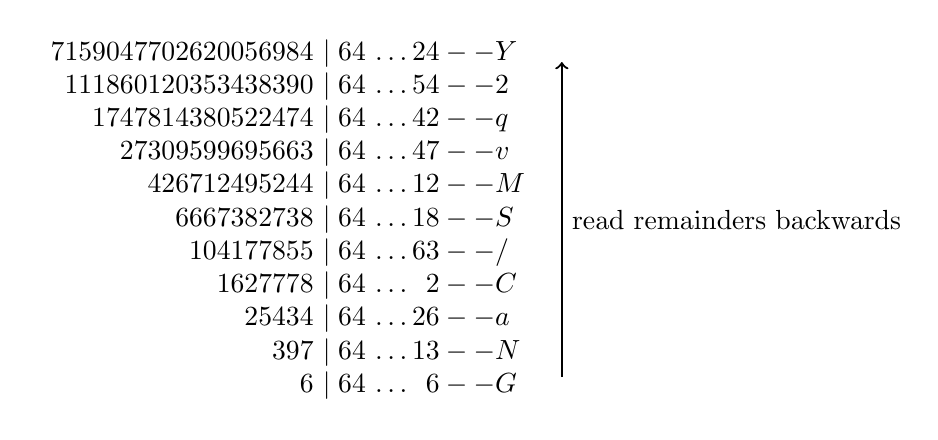
\begin{tikzpicture}[baseline=(current bounding box.center)]
    \node at (0,0) {
        $\begin{array}{r@{~}r@{~}l}
        7159047702620056984 &\mid 64 &\dots 24 -- Y\\
        111860120353438390 &\mid 64 &\dots 54 -- 2\\
        1747814380522474 &\mid 64 &\dots 42 -- q\\
        27309599695663 &\mid 64 &\dots 47 -- v\\
        426712495244 &\mid 64 &\dots 12 -- M\\
        6667382738 &\mid 64 &\dots 18 -- S\\
        104177855 &\mid 64 &\dots 63 -- /\\
        1627778 &\mid 64 &\dots \enspace 2 -- C\\
        25434 &\mid 64 &\dots 26 -- a\\
        397 &\mid 64 &\dots 13 -- N\\
        6 &\mid 64 &\dots \enspace 6 -- G
        \end{array}$
    };
    \draw[->, thick] (current bounding box.east) ++(0.5em,-2cm) -- ++(0, 4.0cm) node[midway,right] {read remainders backwards};
    \end{tikzpicture}
    \end{center}

    So, the base-64 expansion of the natural number $7\,159\,047\,702\,620\,056\,984 = \mathtt{GNaC/SMvq2Y}$.
\end{solutions*}

\begin{chapex}
Let $a, b, c, d \in \mathbb{Z}$. Under what conditions is $(a+b\sqrt{2})(c+d\sqrt{2})$ an integer?
\end{chapex}

\begin{solutions*}
    \[(a+b\sqrt{2})(c+d\sqrt{2}) = ac + 2bd + (ad+bc)\sqrt{2}\]
    Since $a, b, c, d \in \mathbb{Z}$, while $\sqrt{2}$ is irrational, to make $ac + 2bd + (ad+bc)\sqrt{2}$ an integer, $(ad+bc)$ must be $0$. 
    
    Therefore, when $(ad+bc) = 0$, $(a+b\sqrt{2})(c+d\sqrt{2})$ is an integer.
\end{solutions*}

\begin{chapex}
Suppose an integer $m$ leaves a remainder of $i$ when divided by $3$, and an integer $n$ leaves a remainder of $j$ when divided by $3$, where $0 \le i,j < 3$. Prove that $m+n$ and $i+j$ leave the same remainder when divided by $3$.
\end{chapex}

\begin{solutions*}
    According to the problem statement, we have
    \[m = 3k + i \quad \text{ and } \quad n = 3l + j\]
    where $k, l \in \mathbb{Z}$ and $0 \le i,j < 3$.

    \[m+n = (3k + i)+(3l + j) = 3(k+l) + (i+j)\]
    Since $3(k+l)$ is multiple of $3$, so $3(k+l) + (i+j) \equiv (i+j) \pmod 3$. 
    
    Therefore, $m+n$ and $i+j$ leave the same remainder when divided by $3$.
\end{solutions*}

\begin{chapex}
\label{cqRemainderOfSquareMod3}
What are the possible remainders of $n^2$ when divided by $3$, where $n \in \mathbb{Z}$?
\end{chapex}

\begin{solutions*}
    This is the Proposition 1.1.18.
    \begin{proof}
    Let $n \in \mathbb{Z}$. By the division theorem, one of the following must be true for some $k \in \mathbb{Z}$:
    \[
    n=3k \quad \text{or} \quad n=3k+1 \quad \text{or} \quad n=3k+2
    \]
    \begin{itemize}
    \item Suppose $n=3k$. Then
    \[
    n^2 = (3k)^2 = 9k^2 = 3 \cdot (3k^2)
    \]
    So $n^2$ leaves a remainder of $0$ when divided by $3$.
    \item Suppose $n=3k+1$. Then
    \[
    n^2 = (3k+1)^2 = 9k^2+6k+1 = 3(3k^2+2k)+1
    \]
    So $n^2$ leaves a remainder of $1$ when divided by $3$.
    \item Suppose $n=3k+2$. Then
    \[
    n^2 = (3k+2)^2 = 9k^2+12k+4 = 3(3k^2+4k+1)+1
    \]
    So $n^2$ leaves a remainder of $1$ when divided by $3$.
    \end{itemize}
    In all cases, $n^2$ leaves a remainder of $0$ or $1$ when divided by $3$.
    \end{proof}
\end{solutions*}

\begin{definition}
A set $X$ is \textbf{closed} under an operation $\odot$ if, whenever $a$ and $b$ are elements of $X$, $a \odot b$ is also an element of $X$.
\end{definition}

In \Crefrange{cqClosureOfNumberSetsBegin}{cqClosureOfNumberSetsEnd}, determine which of the number sets $\mathbb{N}$, $\mathbb{Z}$, $\mathbb{Q}$ and $\mathbb{R}$ are closed under the operation $\odot$ defined in the question.

\begin{multicols}{2}
\begin{chapex}
\label{cqClosureOfNumberSetsBegin}
$a \odot b = a + b$
\end{chapex}

\begin{chapex}
$a \odot b = a - b$
\end{chapex}

\begin{chapex}
$a \odot b = (a-b)(a+b)$
\end{chapex}

\begin{chapex}
$a \odot b = (a-1)(b-1) + 2(a+b)$
\end{chapex}

\begin{chapex}
$a \odot b = \dfrac{a}{b^2+1}$
\end{chapex}

\begin{chapex}
\label{cqClosureOfNumberSetsEnd}
$a \odot b = \dfrac{a}{\sqrt{b^2+1}}$
\end{chapex}

%\begin{chapex}
%$a \odot b = \begin{cases} a^{b} & \text{if $b > 0$} \\ 0 & \text{if $b \not\in \mathbb{Q}$} \end{cases}$
%% To do: change this - it doesn't make sense
%\end{chapex}
\end{multicols}

\begin{solutions*}
    \fixlistskip
    \begin{center}
    \begin{tabular}{| l | c | c | c | c |}
        \hline
         & $\mathbb{N}$ & $\mathbb{Z}$ & $\mathbb{Q}$ & $\mathbb{R}$ \\
        \hline
        $a \odot b = a + b$ & Yes & Yes & Yes & Yes \\
        \hline
        $a \odot b = a - b$ & No & Yes & Yes & Yes \\
        \hline
        $a \odot b = (a-b)(a+b)=a^2-b^2$ & No & Yes & Yes & Yes \\
        \hline
        $a \odot b = (a-1)(b-1) + 2(a+b)=(a+1)(b+1)$ & Yes & Yes & Yes & Yes \\
        \hline
        $a \odot b = \dfrac{a}{b^2+1}$ & No & No & Yes & Yes \\
        \hline
        $a \odot b = \dfrac{a}{\sqrt{b^2+1}}$ & No & No & No & Yes \\
        \hline
    \end{tabular}
    \end{center}
\end{solutions*}

%\begin{definition}
%A complex number $\alpha$ is \textbf{algebraic} if $p(\alpha) = 0$ for some nonzero polynomial $p(x)$ over $\mathbb{Q}$.
%\end{definition}
%
%\begin{chapex}
%Let $x$ be a rational number. Prove that $x$ is an algebraic number.
%\end{chapex}
%
%\begin{chapex}
%Prove that $\sqrt{2}$ is an algebraic number.
%\end{chapex}
%
%\begin{chapex}
%Prove that $\sqrt{2} + \sqrt{3}$ is an algebraic number.
%\end{chapex}
%
%\begin{chapex}
%Prove that $x+yi$ is an algebraic number, where $x$ and $y$ are any two rational numbers.
%\end{chapex}

\subsection*{True--False questions}

\tfquestiontext{cqGettingStartedTFBegin}{cqGettingStartedTFEnd}

\begin{chapex} % False
\label{cqGettingStartedTFBegin}
Every integer is a natural number.
\end{chapex}

\begin{solutions*}
    \textbf{False}

    Because $\mathbb{N} \subset \mathbb{Z}$, not all integers are natural numbers.
\end{solutions*}

\begin{chapex} % True
Every integer is a rational number.
\end{chapex}

\begin{solutions*}
    \textbf{True}

    Because $\mathbb{Z} \subset \mathbb{Q}$, all integers are rational numbers.
\end{solutions*}

\begin{chapex} % True
Every integer divides zero.
\end{chapex}

\begin{solutions*}
    \textbf{True}

    Because $\forall n \in \mathbb{Z}, 0 = n \odot 0$, According to the Definition 0.33, every integer divides zero.
\end{solutions*}

\begin{chapex} % True
Every integer divides its square.
\end{chapex}

\begin{solutions*}
    \textbf{True}

    Because $\forall n \in \mathbb{Z}, n^2 = n \odot n$, According to the Definition 0.33, every integer divides its square.
\end{solutions*}


\begin{chapex} % True
The square of every rational number is a rational number.
\end{chapex}

\begin{solutions*}
    \textbf{True}

    Every rational number can be represented as a ratio of two integers $\frac{p}{q}, p,q \in \mathbb{Z}$. Its square is $\frac{p^2}{q^2}$, which is a rational number.
\end{solutions*}

\begin{chapex} % False
The square root of every positive rational number is a rational number.
\end{chapex}

\begin{solutions*}
    \textbf{False}

    We can give a counterexample: $2$ is a positive rational number, but its square root $\sqrt{2}$ is not an irrational number.
\end{solutions*}

\begin{chapex} % False
\label{cqGettingStartedTFEnd}
When an integer $a$ is divided by a positive integer $b$, the remainder is always less than $a$.
\end{chapex}

\begin{solutions*}
    \textbf{False}

    According to the division theorem, $a = qb+r$, where $q, r \in \mathbb{Z}$ and the remainder $0 < r \le |b|$. If $a < 0$, then $r$ is greater than $a$. If $0 \le a < b$, then $r = a$.
\end{solutions*}

%\begin{chapex} % False
%Every quadratic polynomial has two distinct complex roots.
%\end{chapex}

\subsection*{Always--Sometimes--Never questions}

\asnquestiontext{cqGettingStartedASNBegin}{cqGettingStartedASNEnd}

\begin{chapex} % Always
\label{cqGettingStartedASNBegin}
Let $n,b_1,b_2 \in \mathbb{N}$ with $1 < n < b_1 < b_2$. Then the base-$b_1$ expansion of $n$ is equal to the base-$b_2$ expansion of $n$.
\end{chapex}

\begin{solutions*}
    \textbf{Always}

    Given $1 < n < b_1 < b_2$, we have $n < b_1$ and $n < b_2$. In any base $b>n$, the integer $n$ is represented by a single digit equal to $n$ itself (since $0 \le n < b$). Therefore, the base-$b_1$ expansion of $n$ is the digit $n$, and the base-$b_2$ expansion of $n$ is also the digit $n$. Hence they are identical.
\end{solutions*}

\begin{chapex} % Never
Let $n,b_1,b_2 \in \mathbb{N}$ with $1 < b_1 < b_2 < n$. Then the base-$b_1$ expansion of $n$ is equal to the base-$b_2$ expansion of $n$.
\end{chapex}

\begin{solutions*}
    \textbf{Never}

    Given $1 < b_1 < b_2 < n$, we have $b_1 < n$ and $b_2 < n$. The integer $n$ can be represented as
    \[n = a_n \cdot b_1^n + a_{n-1} \cdot b_1^{n-1} + \cdots + a_1 \cdot b_1 + a_0\]
    \[n = a_n' \cdot b_2^n + a_{n-1}' \cdot b_2^{n-1} + \cdots + a_1' \cdot b_2 + a_0' \] 
    Because $b_1 \ne b_2$, the expansion of $n$ in base $b_1$ and $b_2$ are not the same.
\end{solutions*}

\begin{chapex} % Sometimes
Let $a,b,c \in \mathbb{Z}$ and suppose that $a$ divides $c$ and $b$ divides $c$. Then $ab$ divides $c$.
\end{chapex}

\begin{solutions*}
    \textbf{Sometimes}

    We can give a counterexample: $a=3, b=6, c=12$. Then $a$ divides $c$ and $b$ divides $c$, but $ab$ does not divide $c$.
\end{solutions*}

\begin{chapex} % Always
Let $a,b,c \in \mathbb{Z}$ and suppose that $a$ divides $c$ and $b$ divides $c$. Then $ab$ divides $c^2$.
\end{chapex}

\begin{solutions*}
    \textbf{Always}

    According to the problem statement, we have
    \[c = ma \quad \text{and} \quad c = nb \quad \text{where} \quad m,n \in \mathbb{Z}\]
    Then $c^2 = ma \cdot nb = (mn)\cdot(ab)$, which is a multiple of $ab$.

    Therefore, $ab$ divides $c^2$.
\end{solutions*}

\begin{chapex} % Always
Let $x,y \in \mathbb{Q}$ and let $a,b,c,d \in \mathbb{Z}$ with $cy+d \ne 0$. Then $\dfrac{ax+b}{cy+d} \in \mathbb{Q}$.
\end{chapex}

\begin{solutions*}
    \textbf{Always}

    $x,y \in \mathbb{Q}$, $x, y$ can be represented as $x=\dfrac{p}{q}$ and $y=\dfrac{r}{s}$, where $p,q,r,s \in \mathbb{Z}$. Then
    \[\dfrac{ax+b}{cy+d} = \dfrac{\dfrac{ap}{q}+b}{\dfrac{cr}{s}+d} = \dfrac{\dfrac{ap+bq}{q}}{\dfrac{cr+ds}{s}} = \dfrac{s(ap+bq)}{q(cr+ds)}\]
    Because $a, b,c,d,p,q,r,s \in \mathbb{Z}$, $\dfrac{ax+b}{cy+d}$ is a rational number.
\end{solutions*}

\begin{chapex} % Sometimes
Let $\dfrac{a}{b}$ be a rational number. Then $a \in \mathbb{Z}$ and $b \in \mathbb{Z}$.
\end{chapex}

\begin{solutions*}
    \textbf{Sometimes}

    We can give a counterexample: $\dfrac{\sqrt{2}}{\sqrt{2}} = 1$ is a rational number, but $\sqrt{2}$ is not a integer, even not a rational number.
\end{solutions*}

\begin{chapex} % Sometimes
Let $x \in \mathbb{R}$ and assume that $x^2 \in \mathbb{Q}$. Then $x \in \mathbb{Q}$.
\end{chapex}

\begin{solutions*}
    \textbf{Sometimes}

    We can give a counterexample: Let $x=\sqrt{2}$, $x^2=2$ is a rational number, but $\sqrt{2}$ is not a rational number.
\end{solutions*}

\begin{chapex} % Always
\label{cqGettingStartedASNEnd}
Let $x \in \mathbb{R}$ and assume that $x^2+1 \in \mathbb{Q}$ and $x^5+1 \in \mathbb{Q}$. Then $x \in \mathbb{Q}$.
\end{chapex}

\begin{solutions*}
    \textbf{Always}

    Given that $x^2 + 1 \in \mathbb{Q}$ and $x^5 + 1 \in \mathbb{Q}$, we can immediately deduce that $x^2 \in \mathbb{Q}$ and $x^5 \in \mathbb{Q}$.

    Let $x^2 = a$ and $x^5 = b$. 

    \begin{itemize}
        \item If $a = 0$, then $x = 0$. Since $0$ is a rational number, $x \in \mathbb{Q}$ is true.
        \item If $a \ne 0$, then $x = \dfrac{x^5}{x^4} = \dfrac{x^5}{(x^2)^2}=\dfrac{b}{a^2}$. Since $b \in \mathbb{Q}$, $a^2 \in \mathbb{Q}$, and $a^2 \neq 0$, $x \in \mathbb{Q}$ is true.
    \end{itemize}
    
    Therefore, $x \in \mathbb{Q}$ is always true.
\end{solutions*}

%\begin{chapex} % Always
%Let $p(x) = ax^2+bx+c$ be a polynomial with $a,b,c \in \mathbb{R}$ and $a \ne 0$, and suppose that $u+vi$ be a complex root of $p(x)$ with $v \ne 0$. Then $u-vi$ is a root of $p(x)$.
%\end{chapex}